\chapter{Medical Background}
\label{ch:rworks}

In medical image analysis the challenges are engrossing and so are the rewards \cite{Duncan2000}. When we solve the related problems in this field, we literally can make an impact on the methods of treating and examining illnesses of the humanity. At present, medical imaging is exceedingly contrasting rather than even couple of years ago \cite{Wang2020}. 

Centered on, medical imaging is an immense area to study. Hence, to keep track, I will pick the particular specimens and techniques up.

\section{Image Modalities}
The notion modalities \cite{Seeram2004} stands for designation of images types. For instance, CT modality or MRI modality. 

Each modality outcomes from a different phenomenon of physics, presenting to doctors (radiologists) an alternative view of the patient. The notability of each modality is that the particular image type has its own advantages and disadvantages. All the factors have to be seriously taken into account once choosing type of modality to be issued or investigated for particular problem.

\subsection{X-Ray (X-RAY)}
For the first time the phenomenon as "x-rays" was issued and explored by Wilhelm Roentgen in 1895 year. Roentgen experimented with rays making them passing through wood and further human tissues. He called them \cite{Barker1996} 'x-rays' where 'x' was considered as a place-holder for the unknown.

X-Rays are the form of electromagnetic radiation in the same spectrum as visible light and radio waves. As well as light, x-rays can be considered as energy of x-ray photon. To emulate x-rays, it can be fired high-energy electrons into matter. 

In medical imaging applications, x-rays used to be sent into human tissues with x-rays machine. Along x-rays move through the patient's body they can interact with many atoms along the path. Finally the sum of all such interactions is recorded in the detector. 

In practice, x-ray images are grayscaled, meaning images are 2 dimensional (2D). Image's values range from 0 to 255, whereas 0 value corresponds to the completely dark pixels and 255 corresponds to the completely white pixels.


\subsection{Computed Tomography (CT)}
The idea of computed tomography approach is to resolve a single slice of an object using many x-ray projections. As the gantry rotates, the scanner collects a 1D x-ray at each angle.

\begin{figure}[h]
    \centering 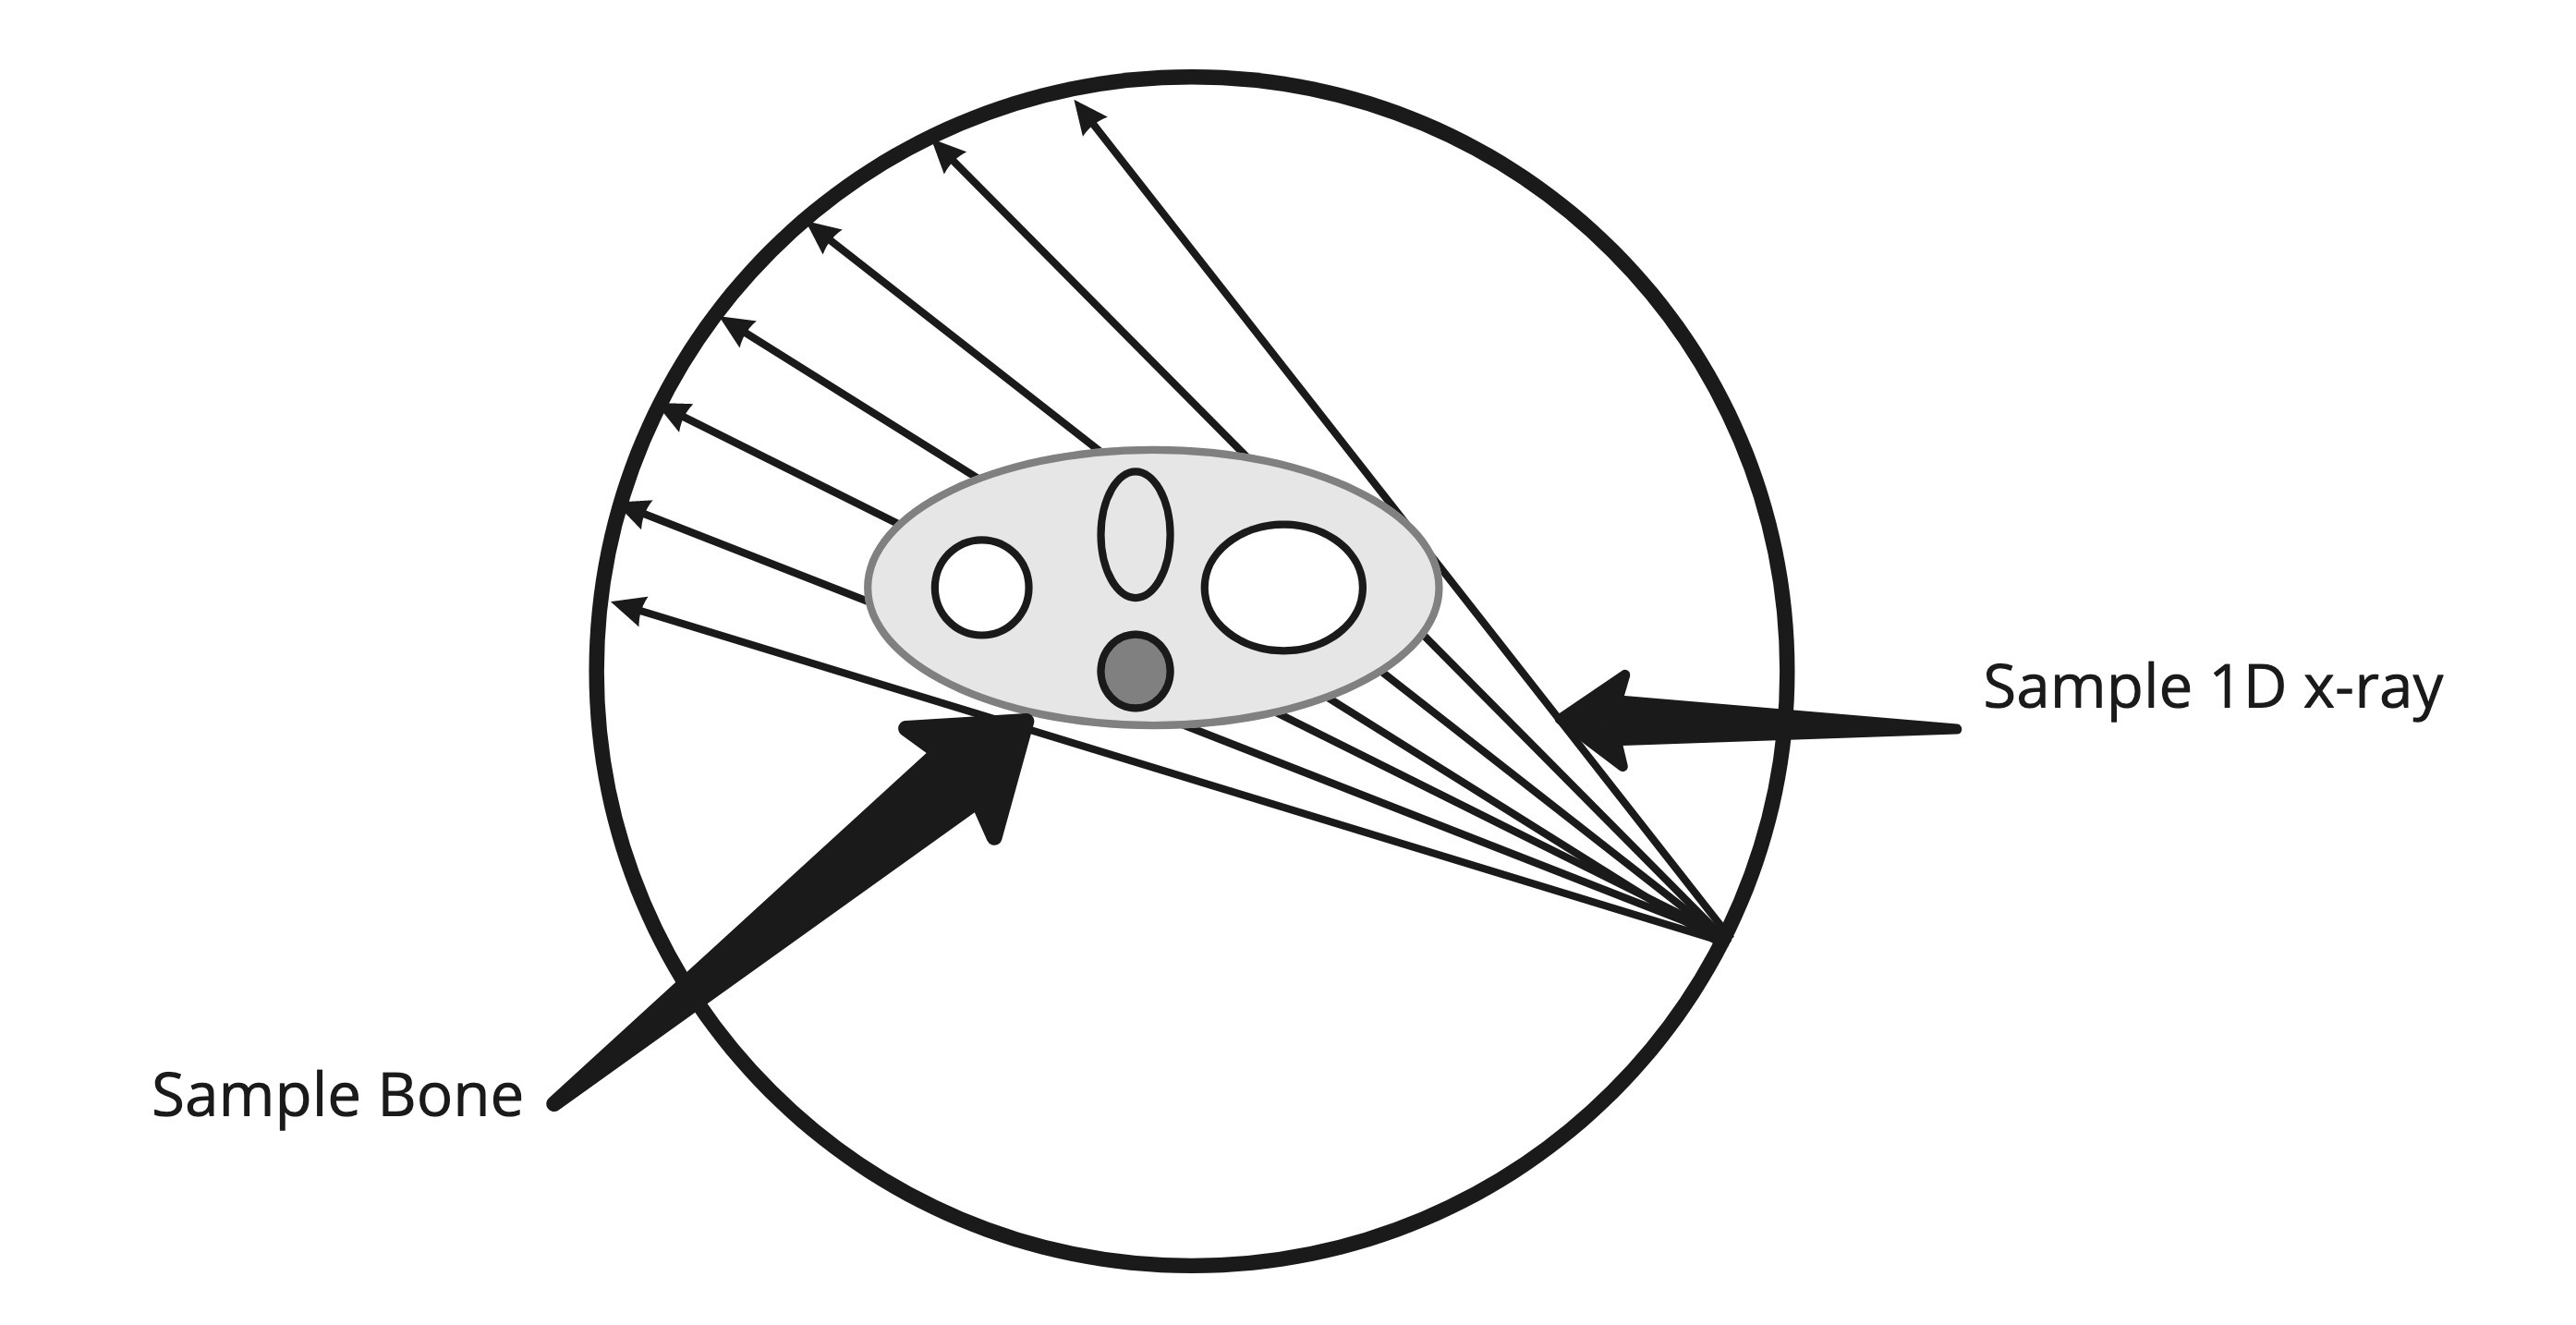
\includegraphics[width=8cm]{images/ct-scan-sample.jpeg}
    \caption {Sample bone CT scan visualisation.}
\end{figure}

CT machine produces images projection which aim to be reconstructed into a 3D volume, which is a scalar field or set of voxels. 

\subsubsection{Contrast Agents}
As one of additional practices jointly CT for retrieving human body information, frequently special substances can be introduced to the body of the patient to add the contrast, what is so called as contrast agents. Often the agents may be essentially useful for visualising of the observations.          

\subsubsection{Motion Artifacts}
The computer tomography result's smoothness depends on whether the patient moved a lot during the acquisition. If so, the resulting transformation will be inconsistent and the reconstructed image will contain errors. But, if the patient's motions are known thereby the artifacts can be corrected during the reconstruction process. As well there are automatic methods which can be applied to sharpen the image by predicting the patient's motions.

The final listcle of the modalities and corresponding practices varies a lot strictly depending of the use case and human body scope of analysis.

\section{Image Reconstruction}
Image reconstruction is a broad and essential field which assumes lot's of research algorithmic involvements. It is significant by the reason of each time the patient is examined the observations should be reconstructed in some mindfully and precise representation extend.    
The field has primary impacts on image quality and hence on radiation dose which certain patient obtains. For a given radiation dose it is desirable to reconstruct images with the lowest possible noise without sacrificing image accuracy and spatial resolution.

In general the procedure to put the projections together to obtain a patient's image is called image reconstruction and can be depicted altogether as shown in Figure \ref{fig:image_reconstruction}.
\begin{figure}[h!]
    \centering 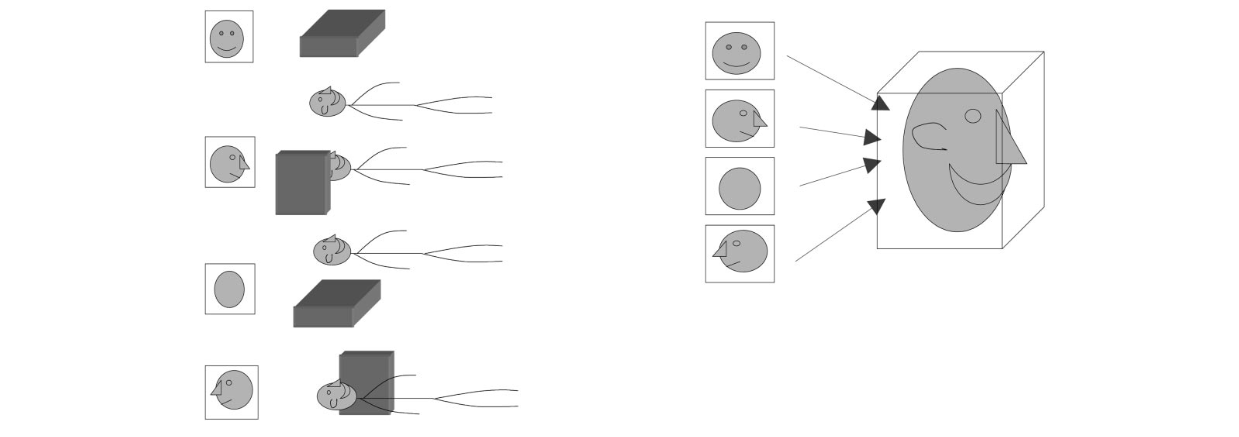
\includegraphics[width=11cm]{images/image_reconstruction.png}
    \caption {Projection data acquired from different views are used to reconstruct the image.}
    \label{fig:image_reconstruction}
\end{figure}

Mainly it is considered two major types of proceeding with reconstruction and they are analytical and iterative accordingly. Talking about CT image reconstruction, it is defined as a mathematical process that forms tomographic images from x-ray projection data which captured at many different angles during receipting the patient.






